\documentclass[11pt]{standalone}
\usepackage{tikz, pgfplots,amsmath, amssymb, amsthm}   
\usepgfplotslibrary{groupplots}


\begin{document}




\tikzset{every picture/.style={line width=0.75pt}} %set default line width to 0.75pt        




\tikzset{every picture/.style={line width=0.75pt}} %set default line width to 0.75pt        

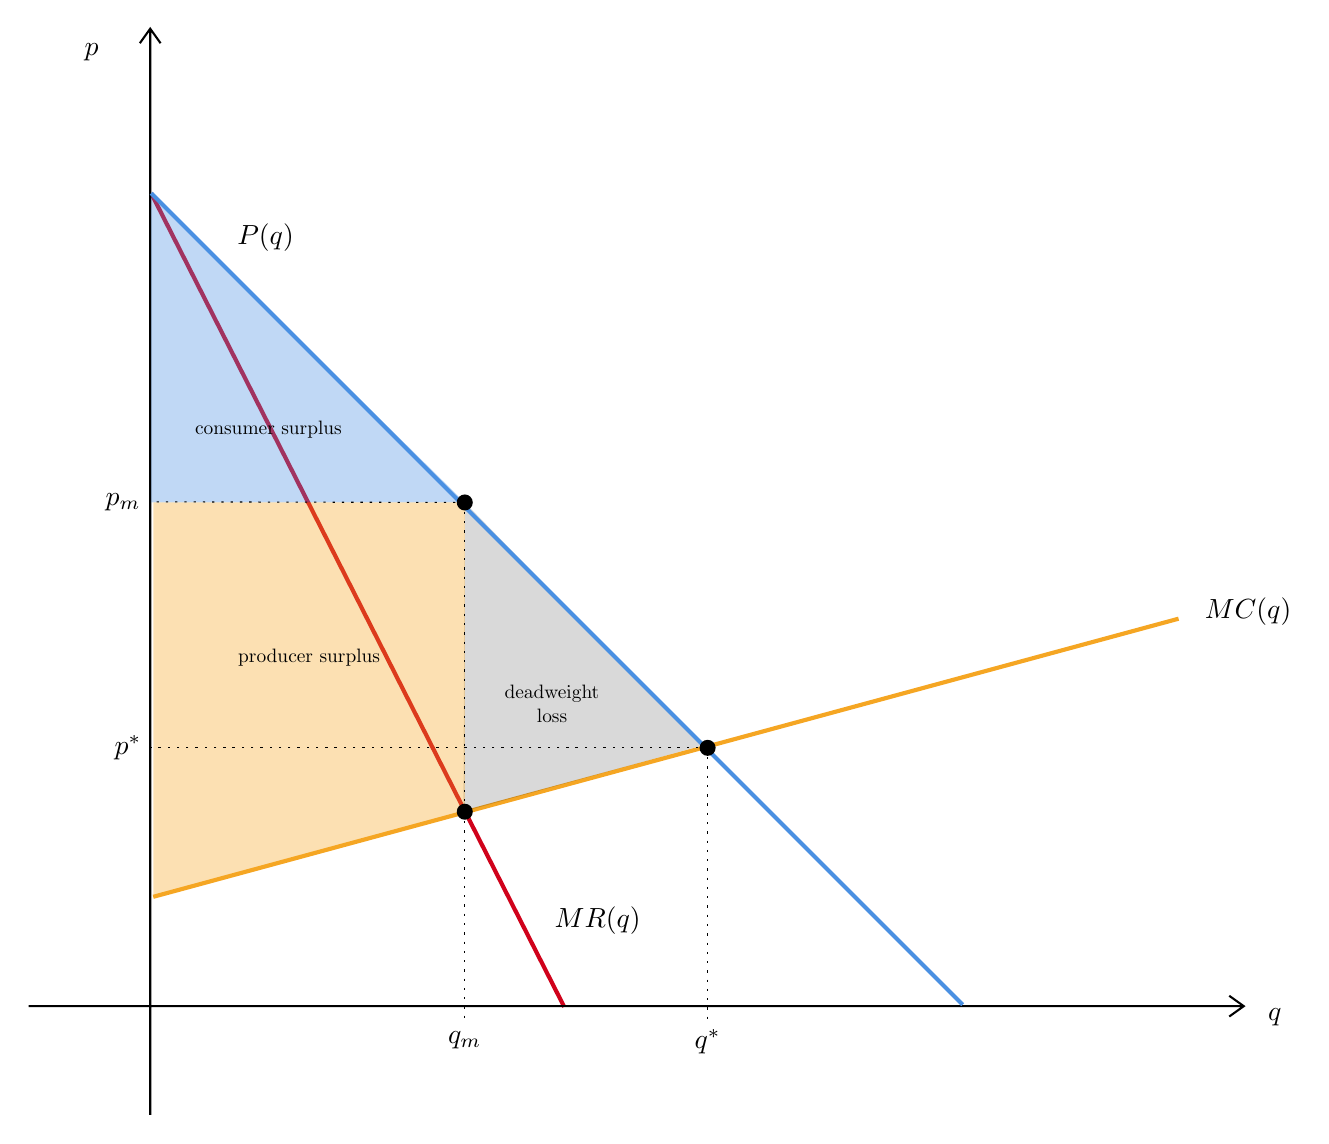
\begin{tikzpicture}[x=0.75pt,y=0.75pt,yscale=-1,xscale=1]
%uncomment if require: \path (0,538); %set diagram left start at 0, and has height of 538

%Straight Lines: MC
\draw [color={rgb, 255:red, 245; green, 166; blue, 35 }  ,draw opacity=1 ][line width=1.5]    (51.5,427) -- (545.5,293) ;


%Straight Lines [id:da306956166359343] 
\draw [color={rgb, 255:red, 208; green, 2; blue, 27 }  ,draw opacity=1 ][line width=1.5]    (50.5,88) -- (249.5,480) ;

%yAxis
\draw [color={rgb, 255:red, 0; green, 0; blue, 0 }  ,draw opacity=1 ][line width=0.75]  (-8.5,479.68) -- (576.91,479.68)(50.04,8.75) -- (50.04,532) (569.91,474.68) -- (576.91,479.68) -- (569.91,484.68) (45.04,15.75) -- (50.04,8.75) -- (55.04,15.75)  ;

%%^ AREAS %%%
%Shape: deadweightloss
\draw  [draw opacity=0][fill={rgb, 255:red, 0; green, 0; blue, 0 }  ,fill opacity=0.15 ] (315.73,354.12) -- (200.91,385.97) -- (201.59,237) -- cycle ;
%Shape: CS
\draw  [draw opacity=0][fill={rgb, 255:red, 74; green, 144; blue, 226 }  ,fill opacity=0.35 ] (50.5,88) -- (201.59,237) -- (50.5,237) -- cycle ;
%Shape: Producer Surplus
\draw  [draw opacity=0][fill={rgb, 255:red, 245; green, 166; blue, 35 }  ,fill opacity=0.35 ] (51.59,237) -- (201.59,237) -- (201.59,387) -- (51.59,427) -- cycle ;
% Text Node
\draw (107,202) node [scale=0.7] [align=left] {consumer surplus};
% Text Node
\draw (126.59,312) node [scale=0.7] [align=left] {producer surplus};
% Text Node
\draw (243.59,334) node [scale=0.7] [align=left] {deadweight\\ \ \ \ \ \ loss};


%Straight Lines [id:da527409949587824] 
\draw  [dash pattern={on 0.84pt off 2.51pt}]  (201.59,237) -- (50.1,236.7) node[anchor=east] {$p_m$};

%Straight Lines [id:da7852562195049779] 
\draw  [dash pattern={on 0.84pt off 2.51pt}]  (201.59,386) -- (201.59,487) node[anchor=north] {$q_m$};



\draw [shift={(201.59,386)}, rotate = 90] [color={rgb, 255:red, 0; green, 0; blue, 0 }  ][fill={rgb, 255:red, 0; green, 0; blue, 0 }  ][line width=0.75]      (0, 0) circle [x radius= 3.35, y radius= 3.35]   ;

%Straight Lines [id:da7170969451112847] 
\draw [color={rgb, 255:red, 74; green, 144; blue, 226 }  ,draw opacity=1 ][line width=1.5]    (50.5,88) -- (441.5,479) ;




%Straight Lines [id:da29337608523799696] 
\draw  [dash pattern={on 0.84pt off 2.51pt}]  (201.59,237) -- (201.59,386) ;

\draw [shift={(201.59,237)}, rotate = 90] [color={rgb, 255:red, 0; green, 0; blue, 0 }  ][fill={rgb, 255:red, 0; green, 0; blue, 0 }  ][line width=0.75]      (0, 0) circle [x radius= 3.35, y radius= 3.35]   ;

% Text Node
\draw (105.62,109.29) node [scale=1]  {$P(q)$};
% Text Node
\draw (591.84,484.92) node {$q$};
% Text Node
\draw (578.96,289.54) node  {$MC(q)$};
% Text Node
\draw (265.62,438.29) node  {$MR(q)$};
% Text Node
\draw (21.84,19.92) node  {$p$};
%Straight Lines [id:da6157081949894307] 
\draw  [dash pattern={on 0.84pt off 2.51pt}]   (318.59,355.22)--(50.5,355.22)   node[anchor=east] {$p^*$};

%Straight Lines [id:da5574885878917746] 
\draw  [dash pattern={on 0.84pt off 2.51pt}]  (318.59,355.22)  --(318.59,486) node[anchor=north] {$q^*$};

\draw [shift={(318.59,355.22)}, rotate = 90] [color={rgb, 255:red, 0; green, 0; blue, 0 }  ][fill={rgb, 255:red, 0; green, 0; blue, 0 }  ][line width=0.75]      (0, 0) circle [x radius= 3.35, y radius= 3.35]   ;


%Straight Lines [id:da7736251371726526] 
% \draw  [dash pattern={on 0.84pt off 2.51pt}]  (50.1,386.7) -- (201.59,387) ;

% \draw [shift={(50.1,386.7)}, rotate = 0.11] [color={rgb, 255:red, 0; green, 0; blue, 0 }  ][line width=0.75]    (-5.59,0) -- (5.59,0)(0,5.59) -- (0,-5.59)   ;




\end{tikzpicture}





\end{document}\textbf{}\textbf{}